

%334% 
$$ asdasd $$
\chapter{Validação \& Verificação}


O desenvolvimento de softwares de simulação, seja utilizando o MEF ou não, é sempre acompanhado de uma bateria de testes, além de um procedimento de validação e verificação (V \& V), que garante, dentro de uma margem de abrangência do que se propõe, sua capacidade de reproduzir resultados concisos, sendo, então, um espelho da realidade.

Verificação, dentro desse contexto, é o procedimento pelo qual se evidencia a exata implementação do modelo matemático no próprio software, ou seja, a verificação que a modelagem programada é equivalente ao algoritmo matemático, dentro dos limites impostos pela aritmética computacional em relação às operações em ponto flutuante\footnote{No computador, os números ditos Reais ($\mathbb{R}$) são representandos por um ponto flutuante, que é uma forma discreta, pois os computadores são desenvolvidos em lógica booleana}. Já a validação, por sua vez, é o processo para determinar a acurácia que um modelo computacional possui de presentar a realidade, dentro dos limites que se propõe. Essas definições estão de acordo com o documento \emph{An Overview of the Guide for Verification and Validation
in Computational Solid Mechanics}, referente a norma ASME respectiva.

Por questões de simplificação, a verificação foi realizada por comparação com outro programa que realiza a mesma análise, o Abaqus, e a validação, por comparação com resultados analíticos, já consolidados experimentalmente.

\section{Verificação}

Para verificar os resultados foram utilizados seis sequências de comparação (três com o elemento tetraédrico, e três triangulares), nas quais aplicaram-se todas as condições de contorno (deslocamentos prescritos, carregamentos pontuais, em linhas e superficiais). Os resultados foram comparados com os obtidos no Abaqus, nas mesmas condições de contorno e geometrias, para deslocamentos nodais e tensões sobre os elementos. As geometrias empregadas foram simples, com malhas pouco refinadas, a fim de facilitar a comparação sobre todos os nós e elementos. 

Os arquivos de verificação estão disponíveis no repositório do projeto, no pasta \emph{verification}, na qual constam os arquivos de entrada do Abaqus (\emph{.cae}) e do GID (\emph{.gid}), além dos arquivos respectivos arquivos de saída, (\emph{.rpt} e \emph{.post.res})

Em todos os casos, definiu-se o aço ASIS 4340 como material, cujas características físicas empregadas aqui foram: $E = 210 \text{GPa}$ (módulo de elasticidade) e $\nu = 0.3$ (coeficiente de Poisson).

Primeiramente, o problema é definido no Abaqus, para depois ser exportado para o GID, a fim de se manter tanto a geometria como a malha, principalmente, as identificações dos nós e elementos, o que facilitada a comparação dos resultados. O procedimento empregado em todos os casos foi o seguinte:

\begin{enumerate}
    \item Definição do problema no Abaqus (\emph{.cae});
    \begin{enumerate}
        \item Construção da geometria;
        \item Definição do material (AISI 4340 STEEL);
        \item Construção da malha;
        \item Definição das condições de contorno;
    \end{enumerate} 
    \item Execução da análise;
    \item Exportação dos resultados para um arquivo de texto (\emph{.rpt});
    \begin{enumerate}
        \item utilização da ferramenta \emph{probe} sobre os nós (deslocamentos nodais);
        \item utilização da ferramenta \emph{probe} sobre os elementos (componentes das tensões e tensão de von Mises);
    \end{enumerate}
    \item Importação do arquivo de \emph{input} no GID (\emph{.inp});
    \item Definição do problema no GID;
    \begin{enumerate}
        \item Definição do material (AISI 4340 STEEL);
        \item Definição das condições de contorno;
    \end{enumerate}
    \item Execução da análise;
    \item Exportação do arquivo de resultados (\emph{.post.res});
    \item Comparação dos resultados.
\end{enumerate}

\subsection{Casos tridimensionais (elemento tetraédrico)}

Nos casos tridimensionais foi empregado a geometria de um cubo unitário, conforme a figura \ref{fig:verificacao_cubo_1}, com a malha descrita na tabela \ref{tab:nos_cubo} e conectividade na tabela \ref{tab:elementos_cubo}. As condições de contorno empregadas foram as seguintes:

\begin{table}
    \centering
    \caption{Descrição dos nós para a malha do cubo unitário.}
    \begin{tabular}{c | c c c}
        \toprule
        \textbf{Nó} & \textbf{x} [m]  & \textbf{y}  [m]  & \textbf{z}  [m]  \\
        \midrule
        1 & 1.000000e+00 & 1.000000e+00 & 1.000000e+00 \\
        2 & 1.000000e+00 & 0.000000e+00 & 1.000000e+00 \\
        3 & 1.000000e+00 & 0.000000e+00 & 0.000000e+00 \\
        4 & 1.000000e+00 & 1.000000e+00 & 0.000000e+00 \\
        5 & 0.000000e+00 & 0.000000e+00 & 1.000000e+00 \\
        6 & 0.000000e+00 & 0.000000e+00 & 0.000000e+00 \\
        7 & 0.000000e+00 & 1.000000e+00 & 0.000000e+00 \\
        8 & 0.000000e+00 & 1.000000e+00 & 1.000000e+00 \\
        9 & 4.929074e-01 & 5.337674e-01 & 5.471772e-01 \\
        \bottomrule
    \end{tabular}
    \label{tab:nos_cubo}
\end{table}

\begin{table}
    \centering
    \caption{Descrição dos nós para a malha do cubo unitário.}
    \begin{tabular}{c | c c c c}
        \toprule
        \textbf{Elemento} & \textbf{Nó 1} & \textbf{Nó 2} & \textbf{Nó 3}  & \textbf{Nó 4} \\
        \midrule
        1 & 2 & 6 & 5 & 9 \\
        2 & 9 & 6 & 5 & 7 \\
        3 & 7 & 9 & 8 & 5 \\
        4 & 6 & 7 & 9 & 3 \\
        5 & 4 & 9 & 1 & 8 \\
        6 & 3 & 4 & 9 & 1 \\
        7 & 3 & 7 & 9 & 4 \\
        8 & 3 & 9 & 2 & 1 \\
        9 & 5 & 9 & 8 & 2 \\
        10 & 9 & 2 & 1 & 8 \\
        11 & 6 & 9 & 2 & 3 \\
        12 & 7 & 9 & 4 & 8 \\
        \bottomrule
    \end{tabular}
\end{table}

\begin{enumerate}
    \item Carregamento superficial (figura \ref{fig:verificacao_cubo_3});
    \item Carregamento pontual (figura \ref{fig:verificacao_cubo_4});
    \item Deslocamento prescrito (figura \ref{fig:verificacao_cubo_5});
\end{enumerate}

\begin{figure}
    \centering
    \caption{O cubo unitário.}
    \begin{subfigure}[b]{0.45\textwidth}
        \centering
        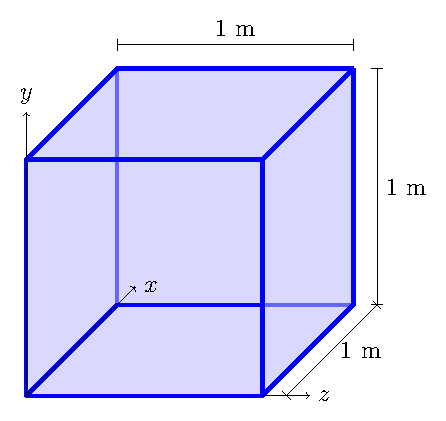
\includegraphics[page=1]{Figuras/verificacao_cubo.pdf}
        \caption{Geometria}
        \label{fig:verificacao_cubo_1}
    \end{subfigure}
    \begin{subfigure}[b]{0.45\textwidth}
        \centering
        \includegraphics[page=2]{Figuras/verificacao_cubo.pdf}
        \caption{Malha}
        \label{fig:verificacao_cubo_2}
    \end{subfigure}
\end{figure}

\begin{figure}
    \centering
    \caption{Condições de contorno para os casos tridimensionais.}
    \begin{subfigure}[b]{0.45\textwidth}
        \centering
        \includegraphics[page=3]{Figuras/verificacao_cubo.pdf}
        \caption{Carregamento superficial}
        \label{fig:verificacao_cubo_3}
    \end{subfigure}
    \begin{subfigure}[b]{0.45\textwidth}
        \centering
        \includegraphics[page=4]{Figuras/verificacao_cubo.pdf}
        \caption{Carga concentrada}
        \label{fig:verificacao_cubo_4}
    \end{subfigure}
    \begin{subfigure}[b]{0.45\textwidth}
        \centering
        \includegraphics[page=5]{Figuras/verificacao_cubo.pdf}
        \caption{Deslocamento prescrito}
        \label{fig:verificacao_cubo_5}
    \end{subfigure}
\end{figure}
